
\section{Results}

Figure~\ref{fig:results} shows the best, average, and worst genome fitness in the population over 300 generations for a single run of the algorithm. Since the optimal fitness value is a minimum, and larger fitness values mean a ``worse'' genome, we negate every fitness value to obtain a more intuitive graph with the minimum at the top. Results seem fairly typical for a genetic algorithm. Worst fitness values are messy and have a high variance across generations. The best fitness values converge fairly quickly and do not vary much. We assume any dips in the best fitness values are due to mutation. At the end of 300 generations, the best genome obtained a fitness of -2734. Using the classical  DP algorithm given this set of keys and frequencies, the actual optimal value is -2837, so this seems fairly close to optimal.

\begin{figure}[h]
    \centering
    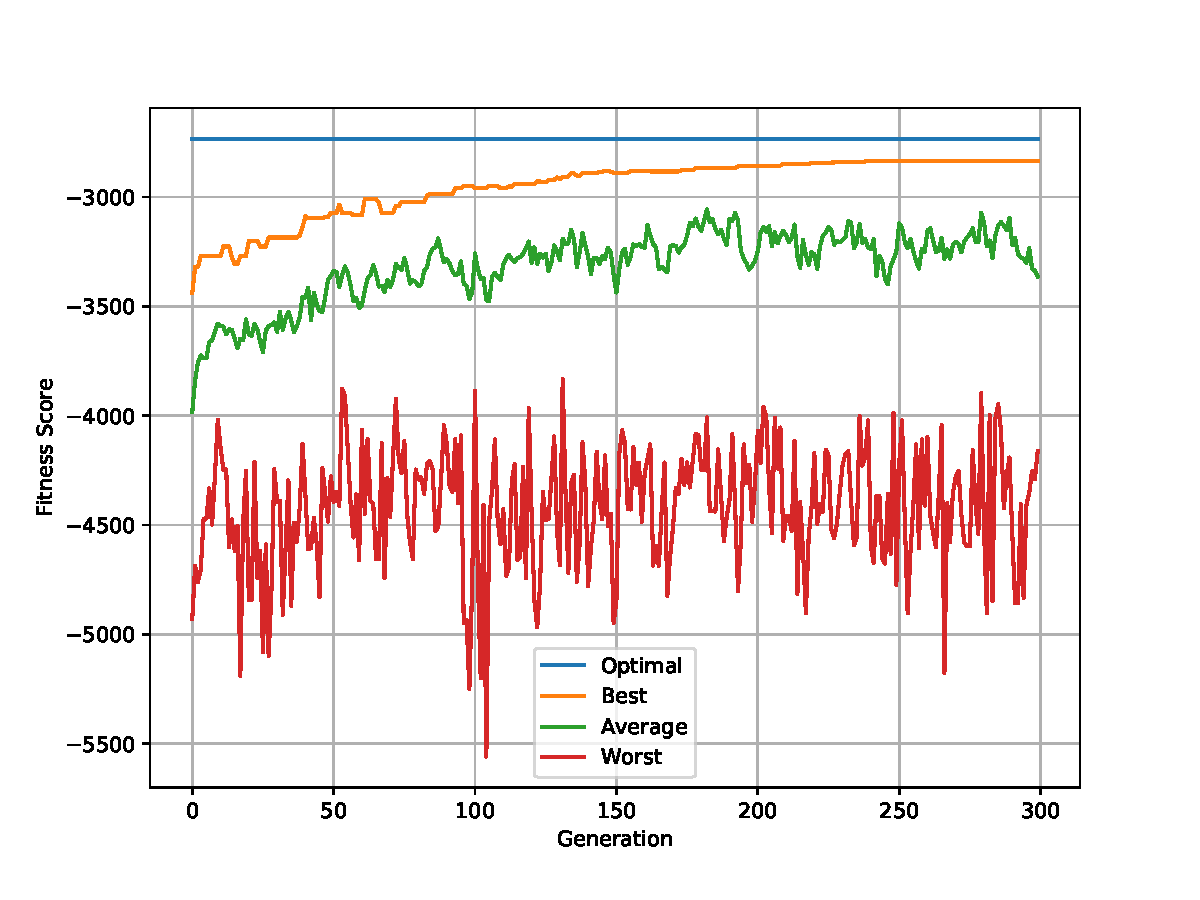
\includegraphics[scale=0.8]{figures/results.pdf}
    \caption{ \small Fitness results over 300 generations. The actual optimal (calculated via DP algorithm) is plotted in blue.}
    \label{fig:results}
\end{figure}
